\chapter{Conception}
\date{}
\section*{Introduction}

Après avoir réalisé l'analyse et la spécification des besoins de la plateforme de pépinière, nous consacrons ce chapitre à la phase de conception du système.
Dans un premier temps, nous présenterons la conception générale à travers la décomposition du système en modules fonctionnels. Ensuite, nous aborderons la conception détaillée en décrivant les différentes classes ainsi que leurs interactions. Enfin, nous illustrerons le fonctionnement du système intelligent à travers des scénarios d'exécution.


\section{Conception générale}

Dans cette partie, nous décomposons notre système de pépinière en plusieurs modules principaux correspondant aux cas d'utilisation identifiés précédemment.

Le système peut être structuré autour des modules suivants :

\subsection*{Gestion des utilisateurs}
Ce module permet la gestion des comptes des différents acteurs de la plateforme (clients, vendeurs, administrateurs).
Il prend en charge l'inscription, l'authentification ainsi que l'activation ou la désactivation des comptes utilisateurs.

\subsection*{Gestion des plantes}
Ce module concerne la gestion des plantes. Il permet l'ajout, la modification et la suppression des plantes par le vendeur ou l'administrateur, ainsi que la consultation de la liste des plantes disponibles à la vente par les clients.

\subsection*{Gestion des commandes}
Ce module permet aux clients de passer des commandes et de suivre leur état.
Il permet également aux vendeurs et administrateurs de consulter les commandes et de les accepter ou les refuser selon la disponibilité du stock.

\subsection*{Module de diagnostic intelligent}
Ce module permet d'assister les utilisateurs dans l'identification des problèmes liés à leurs plantes.
Grâce aux images fournies par l'utilisateur, le système propose un diagnostic ainsi que des recommandations adaptées.

\begin{figure}[h]       % "h" = ici, essaye de garder l'image à cet endroit
    \centering          % centre l'image
    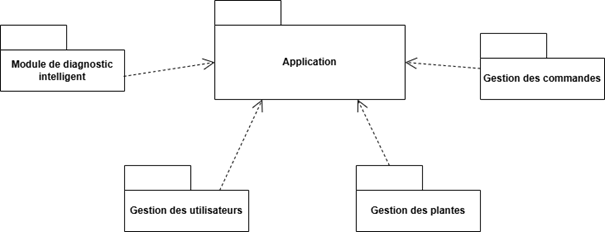
\includegraphics[width=0.8\textwidth]{./image/ImageModule.png}  
    \label{figure: Décomposition modulaire du système} 
    \caption{Décomposition modulaire du système}  % label pour faire référence dans le texte
\end{figure}
\FloatBarrier


\section{Conception détaillée}

Nous allons, dans cette partie, nous focaliser sur la conception détaillée de notre système. Nous ferons recours à l'étude statique et dynamique.

\subsection{Étude statique}

Dans cette section, nous allons présenter les modules de l'application ainsi que les interactions entre les différentes classes.

\subsubsection{Gestion des utilisateurs}
Ce module contient quatre classes : 
Client, Vendeur et Administrateur héritent de la classe Utilisateur.

\begin{itemize}
\item Un administrateur peut gérer plusieurs utilisateurs.
\item Un utilisateur possède un seul rôle dans le système.
\end{itemize}

\begin{figure}[h]       % "h" = ici, essaye de garder l'image à cet endroit
    \centering          % centre l'image
    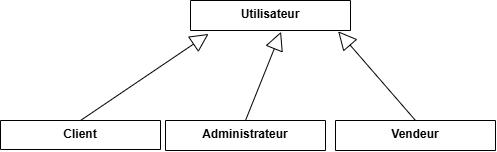
\includegraphics[width=0.7\textwidth]{./image/gestionUtilisateur.png}  
    \label{}   % label pour faire référence dans le texte
    \caption{Composition du module Gestion des utilisateurs}
\end{figure}
\FloatBarrier


\subsubsection{Gestion des plantes}
Ce module contient trois classes : 
Vendeur, Administrateur et Plante.

\begin{itemize}
\item Un vendeur ainsi qu'un administrateur peut ajouter, modifier et supprimer aucune ou plusieurs plantes.
\end{itemize}

\begin{figure}[h]       % "h" = ici, essaye de garder l'image à cet endroit
    \centering          % centre l'image
    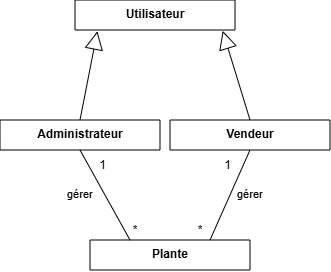
\includegraphics[width=0.5\textwidth]{./image/gestionPlante.png}  
    \label{}   % label pour faire référence dans le texte
    \caption{Composition du module Gestion des plantes}
\end{figure}
\FloatBarrier


\subsubsection{Gestion des commandes}
Ce module contient quatre classes : 
Client, Commande, LigneCommande et Plante.

\begin{itemize}
\item Un client peut passer aucune ou plusieurs commandes.
\item Une commande appartient à un seul client.
\item Une commande est composée d'une ou plusieurs lignes de commande.
\item Une ligne de commande correspond à une seule plante.
\item Une plante peut appartenir à aucune ou plusieurs lignes de commande.
\end{itemize}

\begin{figure}[h]       % "h" = ici, essaye de garder l'image à cet endroit
    \centering          % centre l'image
    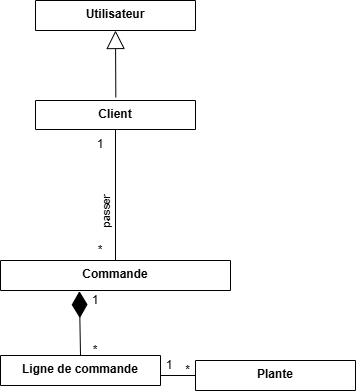
\includegraphics[width=0.5\textwidth]{./image/gestionCommande.png}  
    \label{}   % label pour faire référence dans le texte
    \caption{Composition du module Gestion des commandes}
\end{figure}

\FloatBarrier

\subsubsection{Module de diagnostic intelligent}
Ce module contient quatre classes :
 Client, Diagnostic, ImagePlante et Recommandation AI.

\begin{itemize}
\item Un client peut déposer aucune ou plusieurs imagesPlantes.
\item Un diagnostic est associé à une seule imagePlante.
\item Un diagnostic appartient à un seul client.
\item Une recommandation peut être associée à un ou plusieurs diagnostics.
\end{itemize}

\begin{figure}[h]       % "h" = ici, essaye de garder l'image à cet endroit
    \centering          % centre l'image
    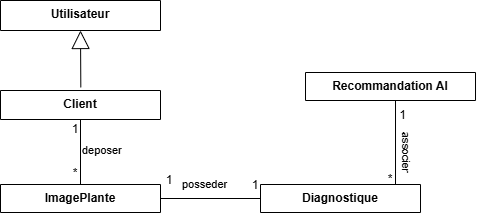
\includegraphics[width=0.7\textwidth]{./image/DiagnosticIntelligent.png}  
    \label{}   % label pour faire référence dans le texte
    \caption{Composition du module Diagnostic intelligent}
\end{figure}
\FloatBarrier

\subsection{Étude des classes}

\begin{figure}[h]       % "h" = ici, essaye de garder l'image à cet endroit
    \centering          % centre l'image
    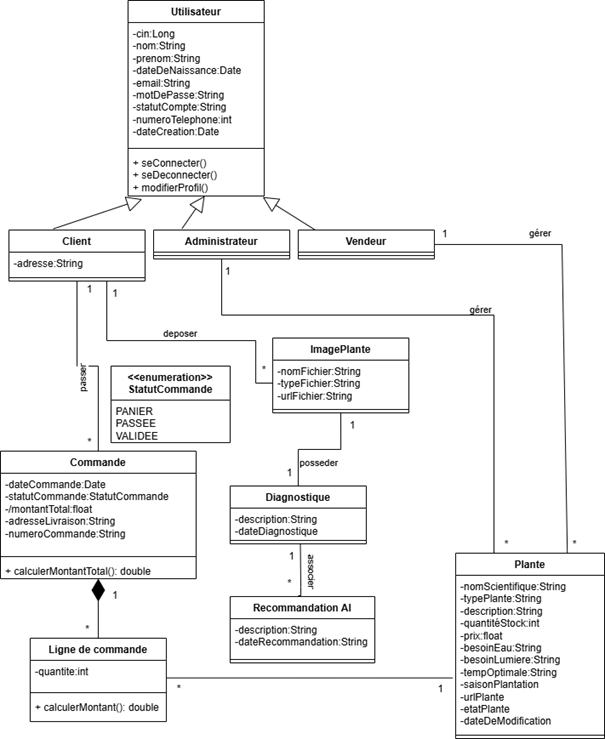
\includegraphics[width=0.8\textwidth]{./image/diagClasse.png}  
    \label{}   % label pour faire référence dans le texte
    \caption{Diagramme de classes}
\end{figure}
\FloatBarrier


Nous nous concentrons sur les classes les plus importantes de notre système et nous
commencerons par la classe utilisateur.
\FloatBarrier
\subsubsection{Classe Utilisateur}

La classe utilisateur est défini par numéro de carte d'identité «cin», un nom « nom », prenom « prénom », date de naissance « dateDeNaissance » , email « email » , mot de passe « motDePasse », statut du compte « statutCompte », numéro de téléphone de l'utilisateur « numeroTelephone » et date de création du compte « dateCréation ».

\begin{figure}[h]       % "h" = ici, essaye de garder l'image à cet endroit
    \centering          % centre l'image
    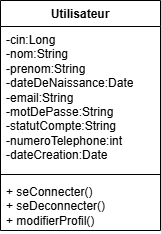
\includegraphics[width=0.3\textwidth]{./image/classeUtilisateur.png}  
    \label{}   % label pour faire référence dans le texte
    \caption{classe Utilisateur}
\end{figure}
\FloatBarrier


\begin{center}
\begin{tabular}{|m{5cm}|m{8cm}|}
\hline
\textbf{Opération} & \textbf{Description} \\
\hline
Se connecter() & Se connecter à l'application \\
\hline
Se déconnecter() & Se déconnecter de l'application \\
\hline
modifierProfil() & Modifier le profil de l'utilisateur \\
\hline
\end{tabular}
\end{center}

\FloatBarrier
\subsubsection{Classe Client}
La classe Client hérite de la classe et représente l'utilisateur qui peut acheter des plantes et demander des diagnostics.
Elle est définie par une adresse « adresse ».

\begin{figure}[h]       % "h" = ici, essaye de garder l'image à cet endroit
    \centering          % centre l'image
    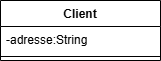
\includegraphics[width=0.3\textwidth]{./image/classeClient.png}  
    \label{}   % label pour faire référence dans le texte
    \caption{classe Client}
\end{figure}

\FloatBarrier

\subsubsection{Classe Vendeur}
La classe Vendeur hérite de Utilisateur et représente l'utilisateur responsable de la gestion des plantes et des commandes.

\begin{figure}[h]       % "h" = ici, essaye de garder l'image à cet endroit
    \centering          % centre l'image
    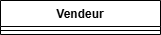
\includegraphics[width=0.3\textwidth]{./image/classeVendeur.png}  
    \label{}   % label pour faire référence dans le texte
    \caption{classe Vendeur}
\end{figure}
\FloatBarrier


\FloatBarrier
\subsubsection{Classe Administrateur}
La classe Administrateur hérite de Utilisateur et permet la gestion globale du système.
\begin{figure}[h]       % "h" = ici, essaye de garder l'image à cet endroit
    \centering          % centre l'image
    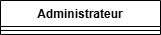
\includegraphics[width=0.3\textwidth]{./image/classeAdmin.png}  
    \label{}   % label pour faire référence dans le texte
    \caption{classe Administrateur}
\end{figure}
\FloatBarrier

\subsubsection{Classe Plante}

La classe Plante est définie par identifiant plante « idPlante », nom scientifique « nomScientifique », type de plante « typePlante », description de la plante « description », quantité disponible en stock « quantitéStock », besoin de la plante en eau « besoinEau », besoin en Lumiere de la plante « besoinLumière », sa température optimale « tempOptimale », la saison de plantation « saisonPlantation », l'image de la plante « urlPlante » et l'état de la plante «etatPlante ».
\begin{figure}[h]       % "h" = ici, essaye de garder l'image à cet endroit
    \centering          % centre l'image
    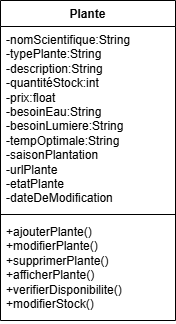
\includegraphics[width=0.3\textwidth]{./image/classePlante.png}  
    \label{}   % label pour faire référence dans le texte
    \caption{classe Plante}
\end{figure}
\FloatBarrier


\begin{center}
\begin{tabular}{|m{5cm}|m{8cm}|}
\hline
\textbf{Opération} & \textbf{Description} \\
\hline
ajouterPlante() & Ajouter une plante \\
\hline
modifierPlante() & Modifier une plante \\
\hline
supprimerPlante() & Supprimer une plante \\
\hline
afficherPlante() & Afficher la liste des plantes \\
\hline
verifierDisponibilite() & Vérifier quantité en stock \\
\hline
modifierStock() & Modifier la quantité en stock \\
\hline
\end{tabular}
\end{center}


\FloatBarrier
\subsubsection{Classe ImagePlante}
La classe ImagePlante est définie par un nom de fichier « nomFichier », un type de fichier «typeFichier » et un url de fichier « urlFichier ».
\begin{figure}[h]       % "h" = ici, essaye de garder l'image à cet endroit
    \centering          % centre l'image
    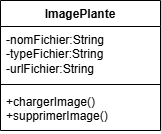
\includegraphics[width=0.3\textwidth]{./image/classeImagePlante.png}  
    \label{}   % label pour faire référence dans le texte
    \caption{classe ImagePlante}
\end{figure}
\FloatBarrier



\begin{center}
\begin{tabular}{|m{5cm}|m{8cm}|}
\hline
\textbf{Opération} & \textbf{Description} \\
\hline
chargerImage() & Charger une image \\
\hline
supprimerImage() & Supprimer une image \\
\hline
\end{tabular}
\end{center}

\FloatBarrier

\subsubsection{Classe Commande}
La classe commande est définie par une date de commande « dateCommande » , statut de la commande « statutCommande », adresse de livraison « adresseLivraison » et le numéro de commande « numeroCommande »
\begin{figure}[h]       % "h" = ici, essaye de garder l'image à cet endroit
    \centering          % centre l'image
    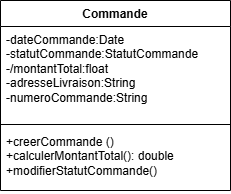
\includegraphics[width=0.4\textwidth]{./image/classeCommande.png}  
    \label{}   % label pour faire référence dans le texte
    \caption{classe Commande}
\end{figure}
\FloatBarrier


\begin{center}
\begin{tabular}{|m{5cm}|m{8cm}|}
\hline
\textbf{Opération} & \textbf{Description} \\
\hline
creerCommande() & Créer une commande \\
\hline
modifierStatutCommande() & Modifier le statut \\
\hline
calculerMontantTotal() & Calculer le montant total \\
\hline
\end{tabular}
\end{center}

\FloatBarrier

\subsubsection{Classe LigneCommande}
La classe Ligne de commande est défini par une quantité <<quantité>>

\begin{figure}[h]       % "h" = ici, essaye de garder l'image à cet endroit
    \centering          % centre l'image
    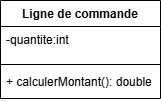
\includegraphics[width=0.3\textwidth]{./image/classeLigneDeCommande.png}  
    \label{}   % label pour faire référence dans le texte
    \caption{classe Ligne de commande}
\end{figure}
\FloatBarrier

\begin{center}
\begin{tabular}{|m{5cm}|m{8cm}|}
\hline
\textbf{Opération} & \textbf{Description} \\
\hline
calculerMontant() & Calculer le montant \\
\hline
\end{tabular}
\end{center}

\FloatBarrier

\subsubsection{Classe Diagnostique}

La classe « Diagnostique » représente le résultat de l'analyse intelligente.
Elle est définie par une description « description » et une date «dateDiagnostique ».

\begin{figure}[h]       % "h" = ici, essaye de garder l'image à cet endroit
    \centering          % centre l'image
    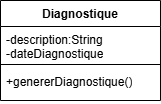
\includegraphics[width=0.3\textwidth]{./image/classeDiagnostique.png}  
    \label{}   % label pour faire référence dans le texte
    \caption{figure: classe Diagnostique}
\end{figure}
\FloatBarrier

\begin{center}
\begin{tabular}{|m{5cm}|m{8cm}|}
\hline
\textbf{Opération} & \textbf{Description} \\
\hline
genererDiagnostic() & Analyser l'image et générer le diagnostic \\
\hline
\end{tabular}
\end{center}

\FloatBarrier

\subsubsection{Classe Recommandation AI}
La classe « Recommandation AI » représente les solutions proposées.
Elle est définie par une description « description » ainsi qu'une date « dateRecommandation ».
\begin{figure}[h]       % "h" = ici, essaye de garder l'image à cet endroit
    \centering          % centre l'image
    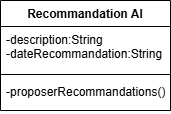
\includegraphics[width=0.3\textwidth]{./image/classeRecommandation.png}  
    \label{}   % label pour faire référence dans le texte
    \caption{classe Recommandation AI}
\end{figure}
\FloatBarrier

\begin{center}
\begin{tabular}{|m{5cm}|m{8cm}|}
\hline
\textbf{Opération} & \textbf{Description} \\
\hline
proposerRecommandations() & Générer les recommandations \\
\hline
\end{tabular}
\end{center}
\FloatBarrier


\section{Description du fonctionnement du diagnostique des plantes}

Après avoir détaillé les méthodes des différentes classes dans l'étude dynamique, nous présentons dans cette section un exemple de scénario intitulé « Diagnostic et recommandation ».
Dans ce scénario, l'utilisateur (client) souhaite obtenir un diagnostic concernant l'état de sa plante à partir d'une image fournie via l'application, ainsi que des recommandations adaptées en fonction du diagnostic établi.
Dans le scénario nominal, le client charge une image de la plante à analyser. Le système transmet ensuite cette image au module de diagnostic intelligent.
Le modèle d'intelligence artificielle intégré à la plateforme (modèle de diagnostic) analyse l'image et génère un diagnostic décrivant le problème détecté (maladie, carence, stress hydrique, etc.).
Dans le cas normal, le système enregistre le diagnostic retourné par le modèle puis le transmet au modèle de recommandation, qui analyse les résultats obtenus et propose des recommandations adaptées, telles que : traitement recommandé, modification des conditions d'arrosage, exposition à la lumière ou utilisation d'un produit spécifique.
Ces recommandations sont ensuite retournées au système, qui les enregistre et les affiche à l'utilisateur afin de l'aider à prendre les actions nécessaires pour améliorer l'état de sa plante.
Dans le scénario d'erreur, si l'image fournie est invalide ou corrompue, le système affiche un message indiquant que le diagnostic n'a pas pu être effectué.
Le résultat affiché par la plateforme sera alors : « Diagnostic indisponible ».



\begin{figure}[h]       % "h" = ici, essaye de garder l'image à cet endroit
    \centering          % centre l'image
    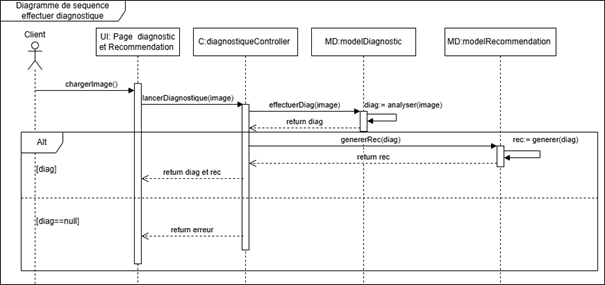
\includegraphics[width=1\textwidth]{./image/diagSequenceAI.png}  
    \label{}   % label pour faire référence dans le texte
    \caption{Diagramme de sequence effectuer diagnostique }
\end{figure}

\FloatBarrier


\section*{Conclusion}

Dans ce chapitre, nous avons présenté la conception générale et détaillée de la plateforme de pépinière en ligne.
La décomposition en modules ainsi que l'étude des classes ont permis de mieux comprendre l'architecture du système et les interactions entre ses composants.
Cette phase de conception constitue une base essentielle pour passer à l'étape suivante, qui est la réalisation et l'implémentation du système.


